\section{Question 1}

\subsection{Question}
\verbatiminput{q1/q1.txt}

\subsection{Answer}
To obtain a basic dataset for this task a list of URIs was required for processing. This list was created using the {\tt get\_uris.py} script. Then, using the {\tt matrix.py} script, the page counts for each blog were extracted and saved to a file called {\tt pagecounts}. The {\tt matrix.py} script is a modified version of {\tt generatefeedvectors.py} from the Programming Collective Intelligence book \cite{pci}. The {\tt get\_uris main} function in Listing \ref{listing:geturis:main} was the driver that called {\tt get\_atom} funciton from Listing \ref{listing:geturis:atom} to extract the atom \cite{atom} formatted blog entries and if one existed for that particular blog it was added to the URIs set for storage with the {\tt add\_uri} function, shown in Listing \ref{listing:geturis:adduri}.

\lstinputlisting[language=Python, caption={main for get\_uris.py}, label=listing:geturis:main, linerange={27-39}, firstnumber=27]{q1/get_uris.py}

\lstinputlisting[language=Python, caption={get\_atom function}, label=listing:geturis:atom, linerange={10-19}, firstnumber=10]{q1/get_uris.py}

\lstinputlisting[language=Python, caption={add\_uri function}, label=listing:geturis:adduri, linerange={21-25}, firstnumber=21]{q1/get_uris.py}


This code uses the value stored in the {\tt default} variable as seed for obtaining random blogs. Using the BeautifulSoup library \cite{py:soup}, the contents of the blog were parsed and if an atom feed was found that link was extracted and then saved as part of the set of URIs in the {\tt blog\_uris} file.

The contents of each blog were downloaded and processed by the code shown in Listing \ref{listing:matrix:get} and the {\tt get\_titles}, {\tt get\_words} and {\tt get\_next} functions found in Listing \ref{listing:matrix:gettitles}. This code loops over the URIs that were downloaded with the {\tt get\_uris.py} script, loops over each entry and extracts all the words in each entry's title. These words were compiled into a master list for all 100 blogs, with the top 500 words that fit into the range bounded by the code in Listing \ref{listing:matrix:bounds}. 

\lstinputlisting[language=Python, caption={looping over the URIs}, label=listing:matrix:get, linerange={40-49}, firstnumber=40]{q1/matrix.py}

\clearpage

\lstinputlisting[language=Python, caption={processing each blog}, label=listing:matrix:gettitles, linerange={8-37}, firstnumber=8]{q1/matrix.py}

\lstinputlisting[language=Python, caption={bounding the terms}, label=listing:matrix:bounds, linerange={70-73}, firstnumber=70]{q1/matrix.py}

To build the histogram the {\tt pagecounts} file was parsed by the R script in Listing \ref{listing:hist} and saved as a pdf, which is shown in Figure \ref{fig:hist}.

\lstinputlisting[language=R, caption={building the histogram}, label=listing:hist]{q1/build_histogram.r}

\clearpage

\begin{figure}[h!]
\centering
\fbox{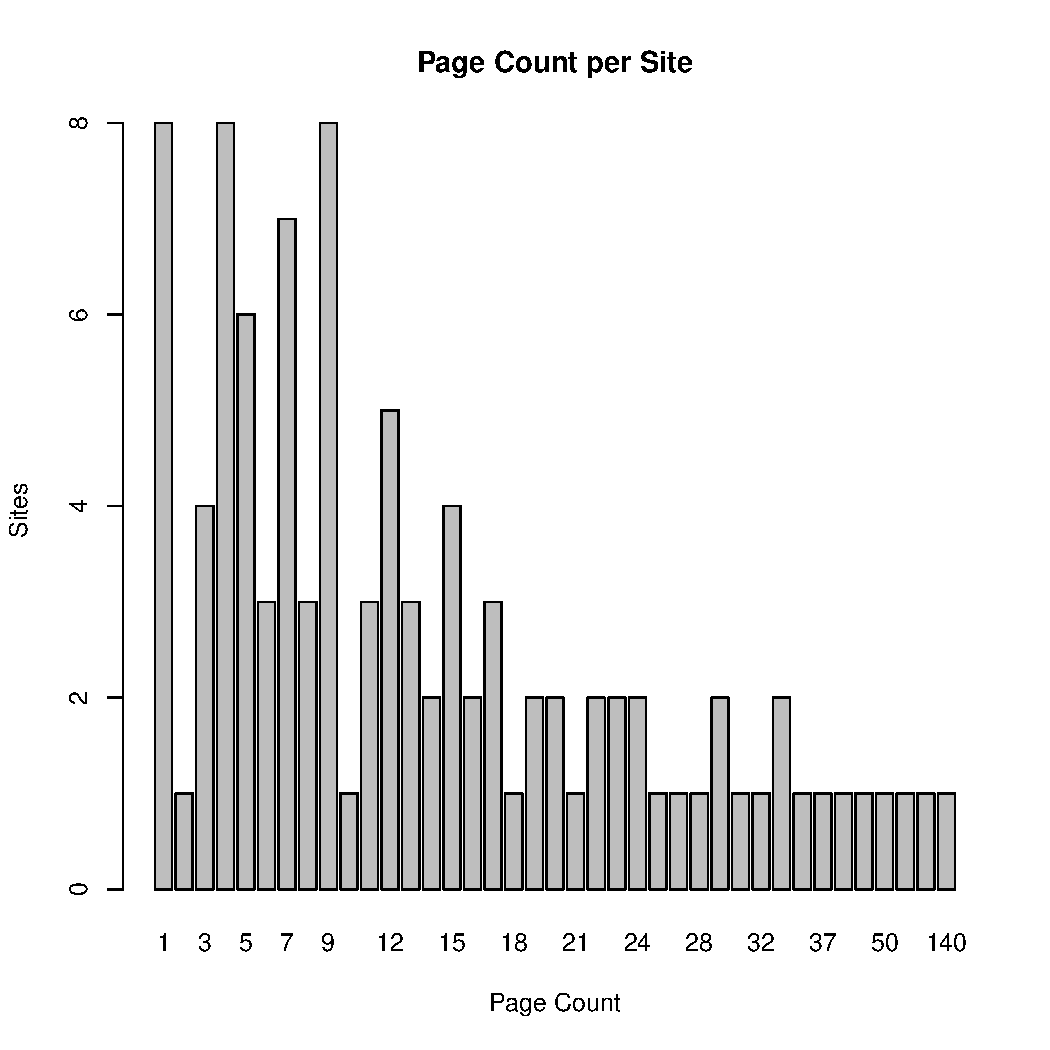
\includegraphics[scale=0.75]{q1/hist.pdf}}
\caption{Page Count per Blog}
\label{fig:hist}
\end{figure}


% \lstinputlisting[language=Python, caption={matrix.py}, label=listing:matrix]{q1/matrix.py}